%!TEX root = ../../../adrien_gomar_phd.tex

As shown above in a single rotor propeller, the outlet velocity is not axial
yielding a residual tangential velocity $\Delta V_{\theta}$,
which forms the swirl. 
This is a lost energy that deteriorates the propulsive efficiency. 
To recover it, a second contra-rotating rotor can be used~\cite{Hager1988}.
We will see in this section through a simple velocity triangle exercise that
the swirl is annulled by the second rotor. 
This allows to create more thrust with the same inflow conditions.
The loading of the blades can thus be reduced compared
to propeller blades, for a given level of thrust.
This increases the propulsive
efficiency for transonic flight conditions
as shown by \citet{Hughes1989} and reported 
in Figure~\ref{fig:hughes_propulsive_efficiency}.
\begin{figure}[htp]
  \centering
  \includegraphics*[width=0.40\textwidth]{hughes_propulsive_efficiency}
  \caption{Benefit of using a contra-rotating open rotor, from \citet{Hughes1989}.}
  \label{fig:hughes_propulsive_efficiency}
\end{figure}

\subsection{Geometry}
\label{sub:cror_geometry}

Figure~\ref{fig:cror_geometry} depicts the main
geometrical parameters of a CROR.
It is composed of two rotors, the first one is called
the front rotor and the second one is called the rear or aft rotor.
Generally, they do not have the same diameter and rotation speed. 
Thus, subscript $f$ and $r$ denotes respectively,
the front and the rear parameters.
The difference of diameter is called the clipping or cropping
of the blades and is evaluated through the non-dimensional parameter
$\kappa$
\begin{equation}
    \kappa = \frac{D_f - D_r}{D_f}.
\end{equation}
By clipping the rear rotor blades, 
tip vortices shed by the front rotor are not likely
to hit the rear rotor.
Finally, the spacing between the rotors
is evaluated as the difference between the axial minimum of the
rear blade minus the axial maximum of the front blade. The spacing
is one of the adjustment parameters used to minimize the unsteady
interaction between the rotors to reduce noise. In fact, 
heterogeneities are lessened along with the convection of
the flow field. These heterogeneities are responsible
for the unsteady interactions and, by extrapolating, for noise generation.
\begin{figure}[htp]
  \centering
  \includegraphics*[scale=0.3]{cror_geometry.pdf}
  \caption{Geometry of a contra-rotating open rotor.}
  \label{fig:cror_geometry}
\end{figure}

Two types of contra-rotating open rotors have emerged. The first
type is the puller configuration, whose blades 
are near the front of the spinner as 
shown in Figure~\ref{fig:cror_configurations}. As the
name indicates, this configuration is mounted in front of the
wing. It is particularly interesting as the blades will see
a uniform flow. However, these all suffer from the same incidence as that
of the wing. This can give large in-plane forces 
(forces normal to the rotation axis~\cite{ThesisFrancois}) compared to pusher
configurations. In opposite, the deflection of the flow due to the wing provides
a smaller incidence.
Moreover, the distortion generated
by the CROR will disturb the flow around the wing. As one way to reduce
consumption of airplanes is to have laminar wings, this configuration
is less studied. The second type is the pusher
configuration. It is designed to be mounted on a pylon which will thus
interact with the CROR, but laminar wings might be considered with
this configuration. In this work, we will deal with a pusher configuration
in Chapters~\ref{cha:dream_ls_isolated} and
\ref{cha:dream_hs_isolated}.
\begin{figure}[htp]
  \centering
  \subfigure[puller]{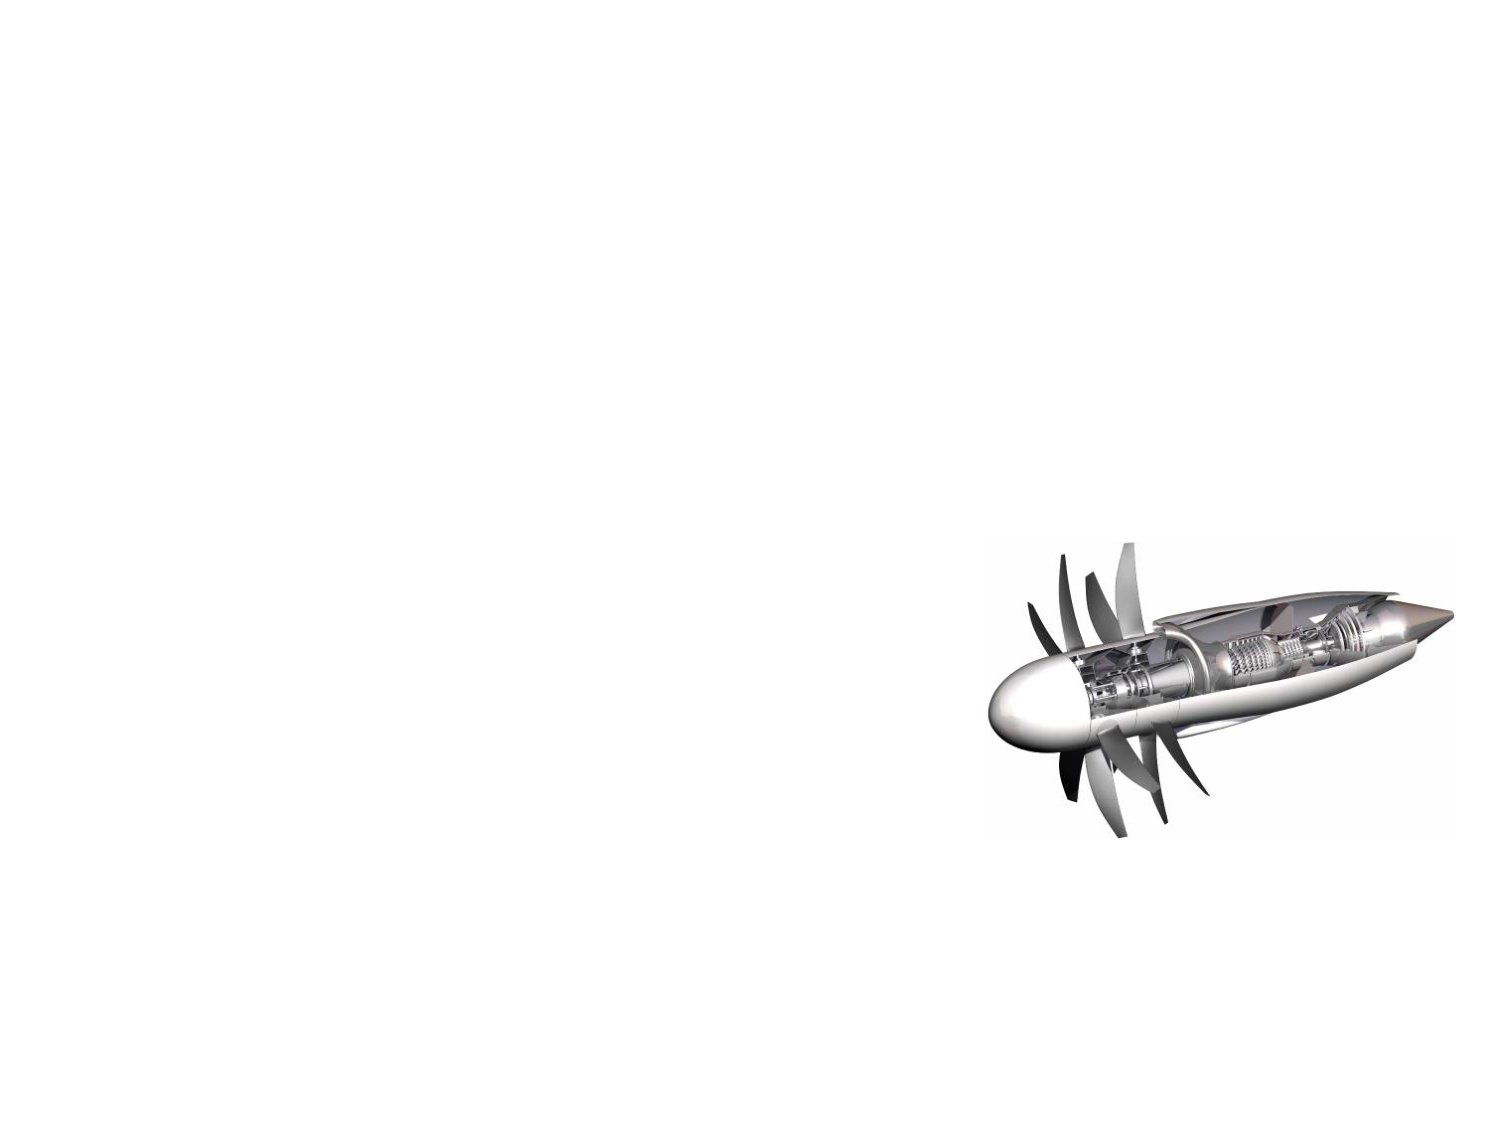
\includegraphics[width=.4\textwidth]{puller.pdf}}
  \subfigure[pusher]{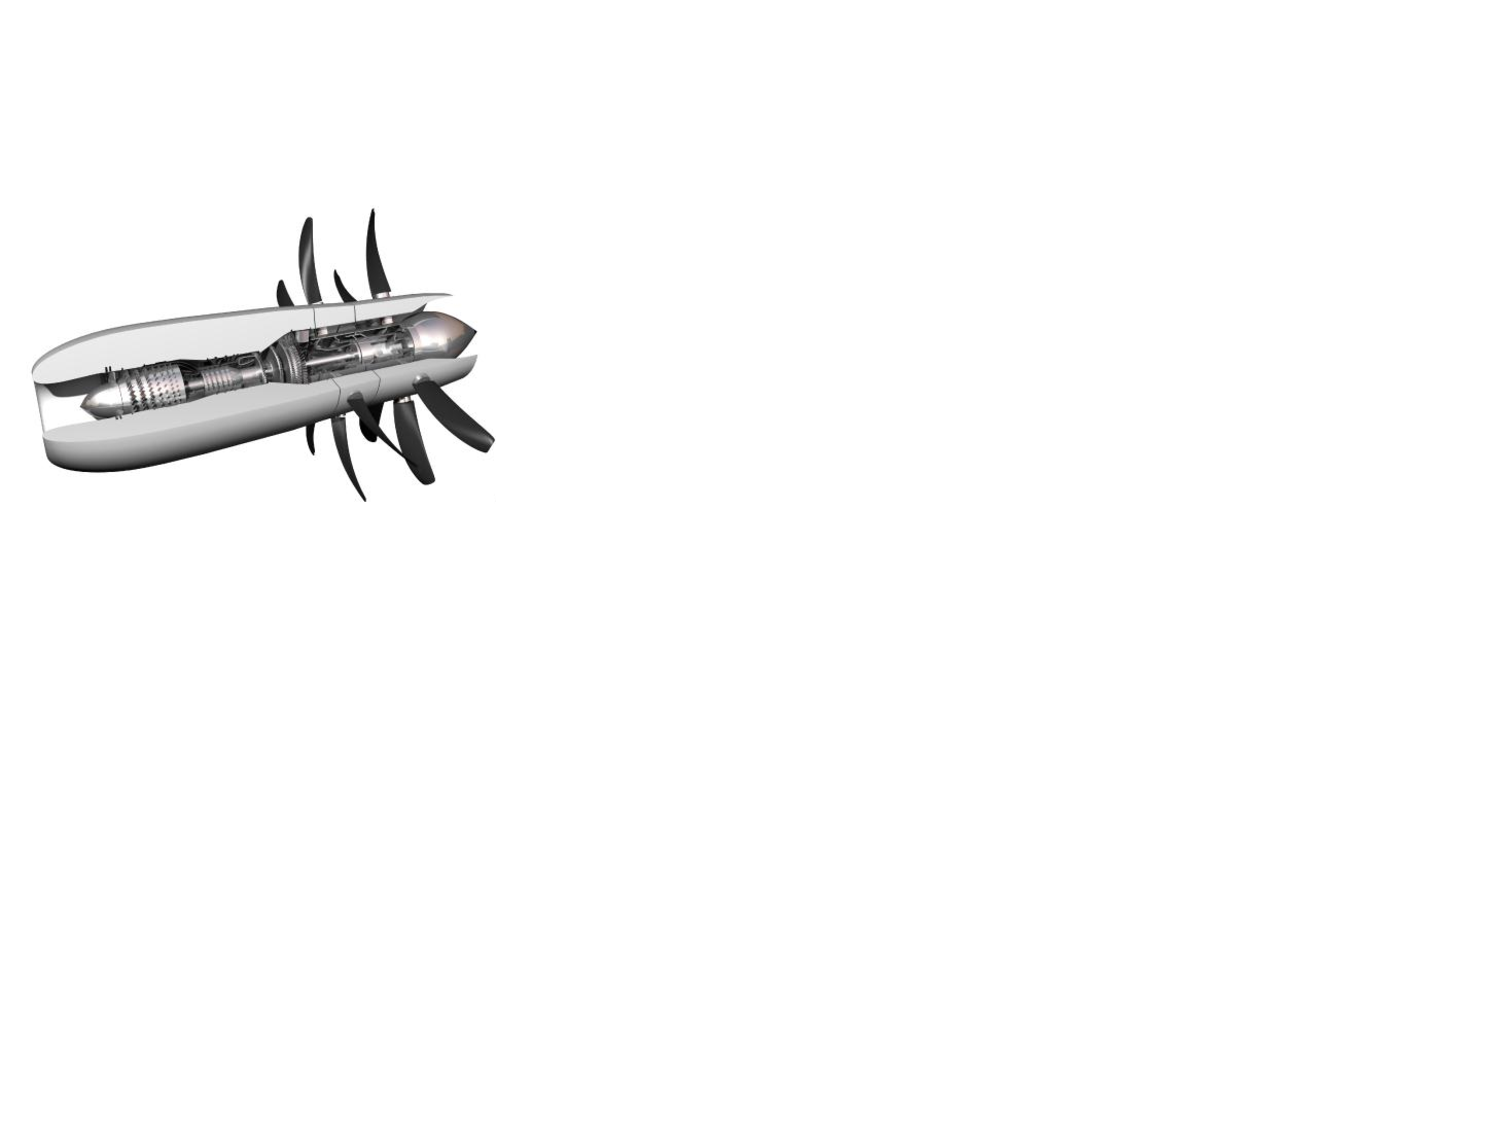
\includegraphics[width=.4\textwidth]{pusher.pdf}}
  \caption{Types of contra-rotating open rotor, courtesy Rolls-Royce.}
  \label{fig:cror_configurations}
\end{figure}
% For pusher CROR, two types of architectures can be thought:
% one based on a gearbox and the second
% being build around a statorless low-pressure turbine. These
% two 
% \begin{figure}[htp]
%   \centering
%   \subfigure[geared design]{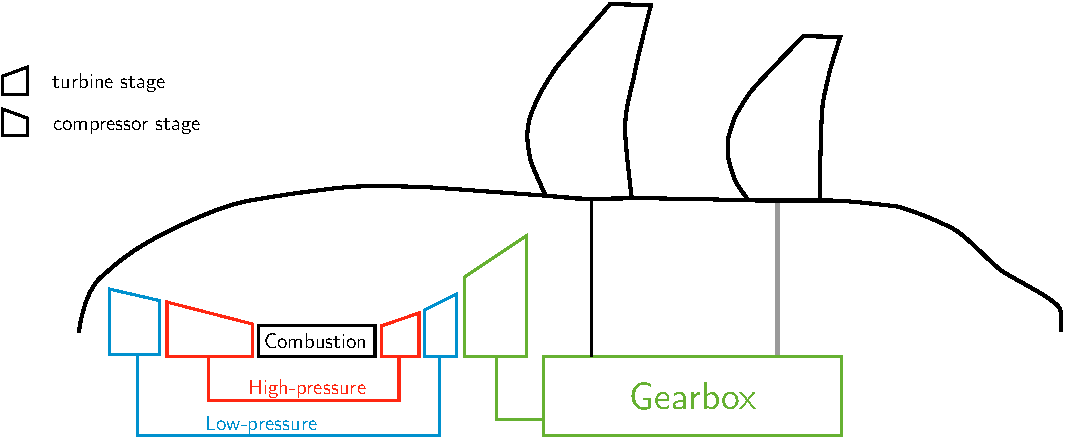
\includegraphics[width=.4\textwidth]{geared_cror.pdf}}
%   \subfigure[statorless low-pressure turbine design]{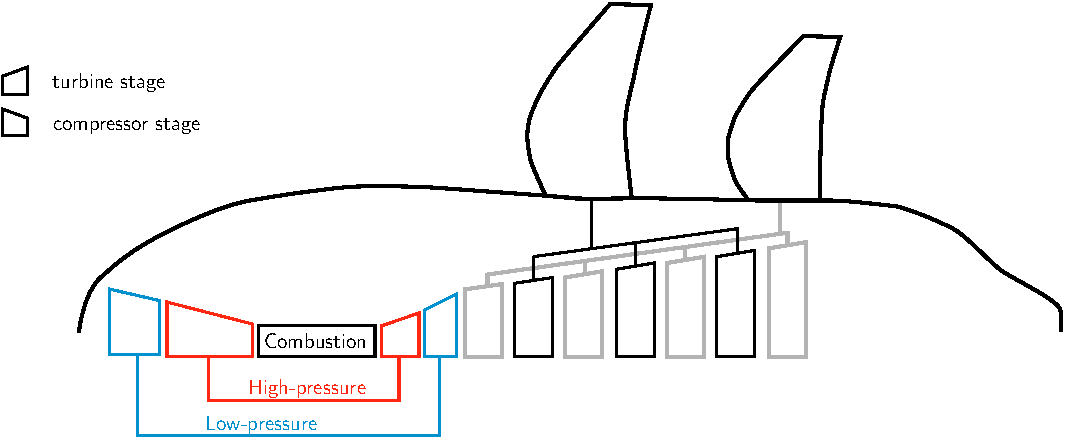
\includegraphics[width=.4\textwidth]{stator_less_cror.pdf}}
%   \caption{Contra-rotating open rotor pusher architectures.}
%   \label{fig:cror_architectures}
% \end{figure}

\subsection{Velocity triangle}
\label{sub:cror_velocity_triangle}
\begin{figure}[htp]
  \centering
  \includegraphics*[scale=0.5]{velocity_triangle_cror.pdf}
  \caption{Velocity triangle applied to a contra-rotating open rotor.}
  \label{fig:velocity_triangle_cror}
\end{figure}
Figure~\ref{fig:velocity_triangle_cror} shows the application
of the velocity triangle to a CROR configuration. The swirl
energy that was lost by the propeller is now used to 
produce more thrust. Therefore, a CROR will finally have a better propulsive
efficiency than a propeller, which explains its study as
a greener engine. In the eighties, 
\citet{Strack1981} and \citet{Hager1988} showed that
using a contra-rotating open rotor technology over
a single propeller gave an increase of $6-8\%$
in propulsive efficiency, explaining its regain of interest.
Today, high-speed propellers blades might lead to higher increase
in efficiency
while keeping a flight Mach number close to $0.8$, enabling its use
for commercial aviation.

\subsection{Similarity coefficients}
\label{sub:cror_similarity_coeff}

In the case of a CROR configuration, the front and the rear rotors 
have to be considered.
Two main ways exist to evaluate the global value of the
similarity coefficients. The first one, chosen by
\citet{Bechet2011} among others, is to consider
that the non-dimensional parameter $D$, $n$ and $J$ are those
of the front rotor for both rotors
\begin{equation}
    J_f = J_r = \frac{V_0}{n_f D_f}, \quad
    C_T = \frac{F_{x_f} + F_{x_r}}{\rho_f n_f ^ 2  D_f ^ 4}, \quad
    C_P = \Omega_f \frac{M_{x_f} + M_{x_r}}{\rho_f n_f ^ 3 D_f ^ 5}, \quad
    \eta = J_f \frac{C_T}{C_P}.
\end{equation} 
The second one uses the non-dimensional parameter of the current rotor,
as done by \citet{Stuermer2008} and \citet{Zachariadis2011}.
The first approach is retained for the current work as it allows
to simplify the comparison of the similarity coefficient with equivalent propellers.
